\subsection{Data Visualisation} 
% Data visualization
Data visualisation is concerned with displaying graphical representations of the data. To gain further understanding into the provided data, it is also possible to visualise the different floors of the sites. 

\begin{figure}[H]
    \centering
    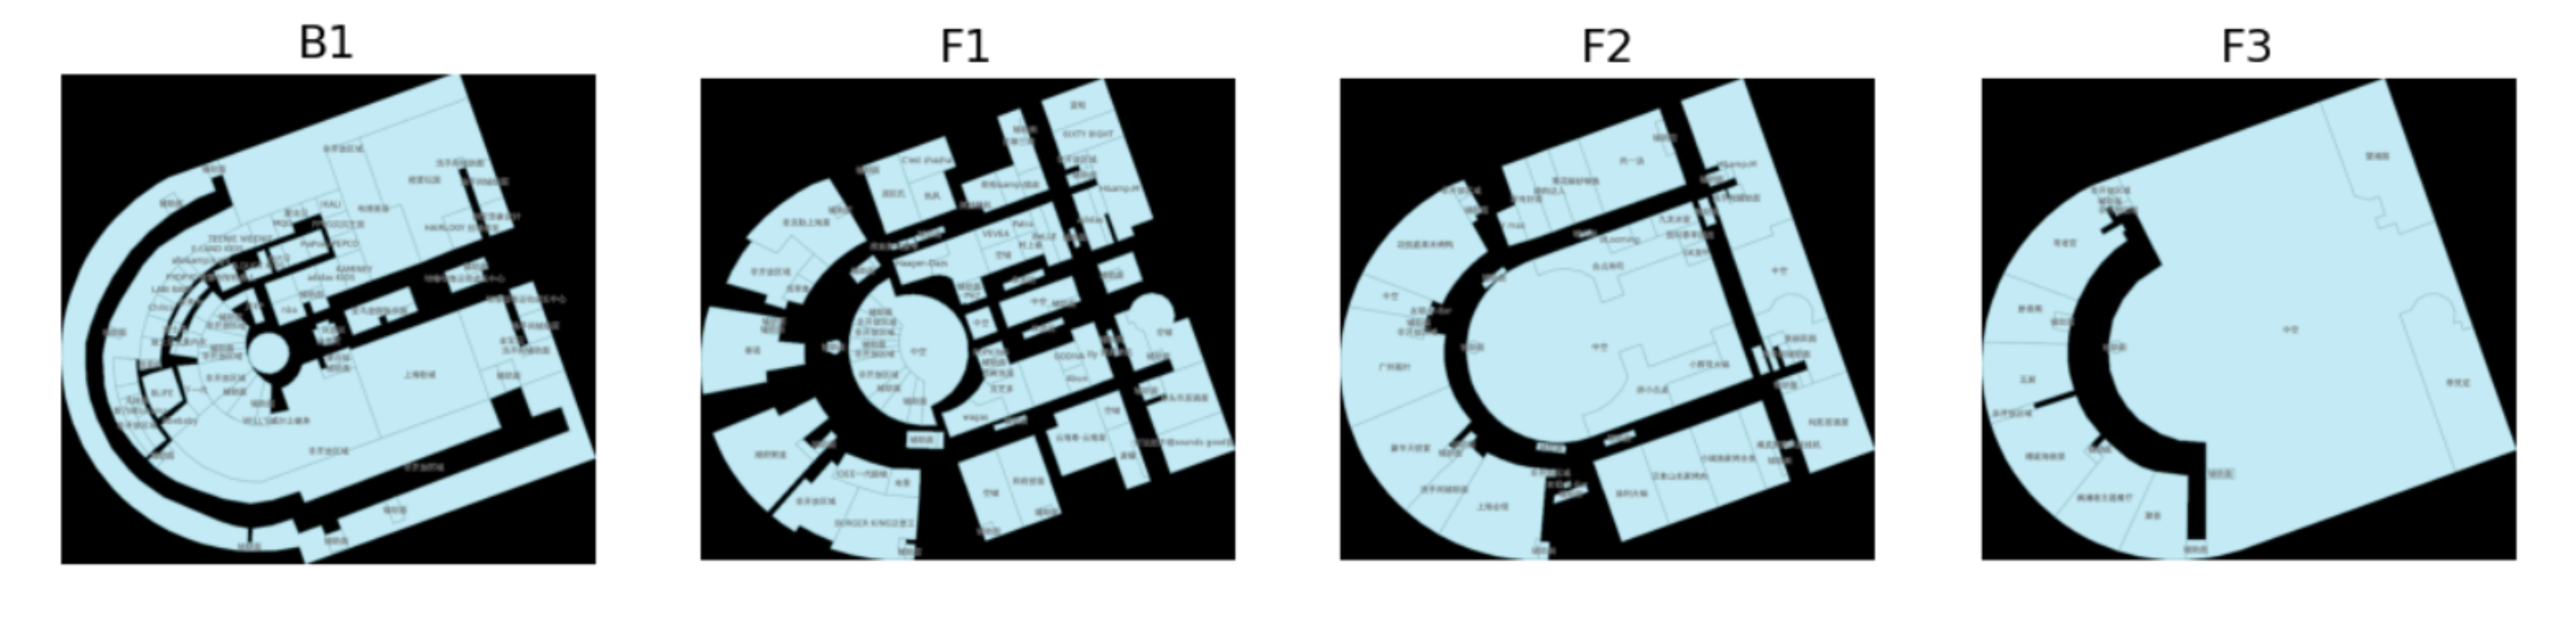
\includegraphics[scale=.31]{Images/ProblemAnalysis/datavisual.png}
    \caption{Depiction of the different floors at a particular site.}
    \label{fig:datavisual}
\end{figure}

Seen on \textbf{\autoref{fig:datavisual}} is an example of a site with its different levels. Level names starting with a B indicates a basement level, where levels starting with F indicates a regular floor. The number indicates the number of levels to the ground from the particular level. The different sites vary a lot in terms of the number of levels.

\begin{figure}[H]
    \centering
    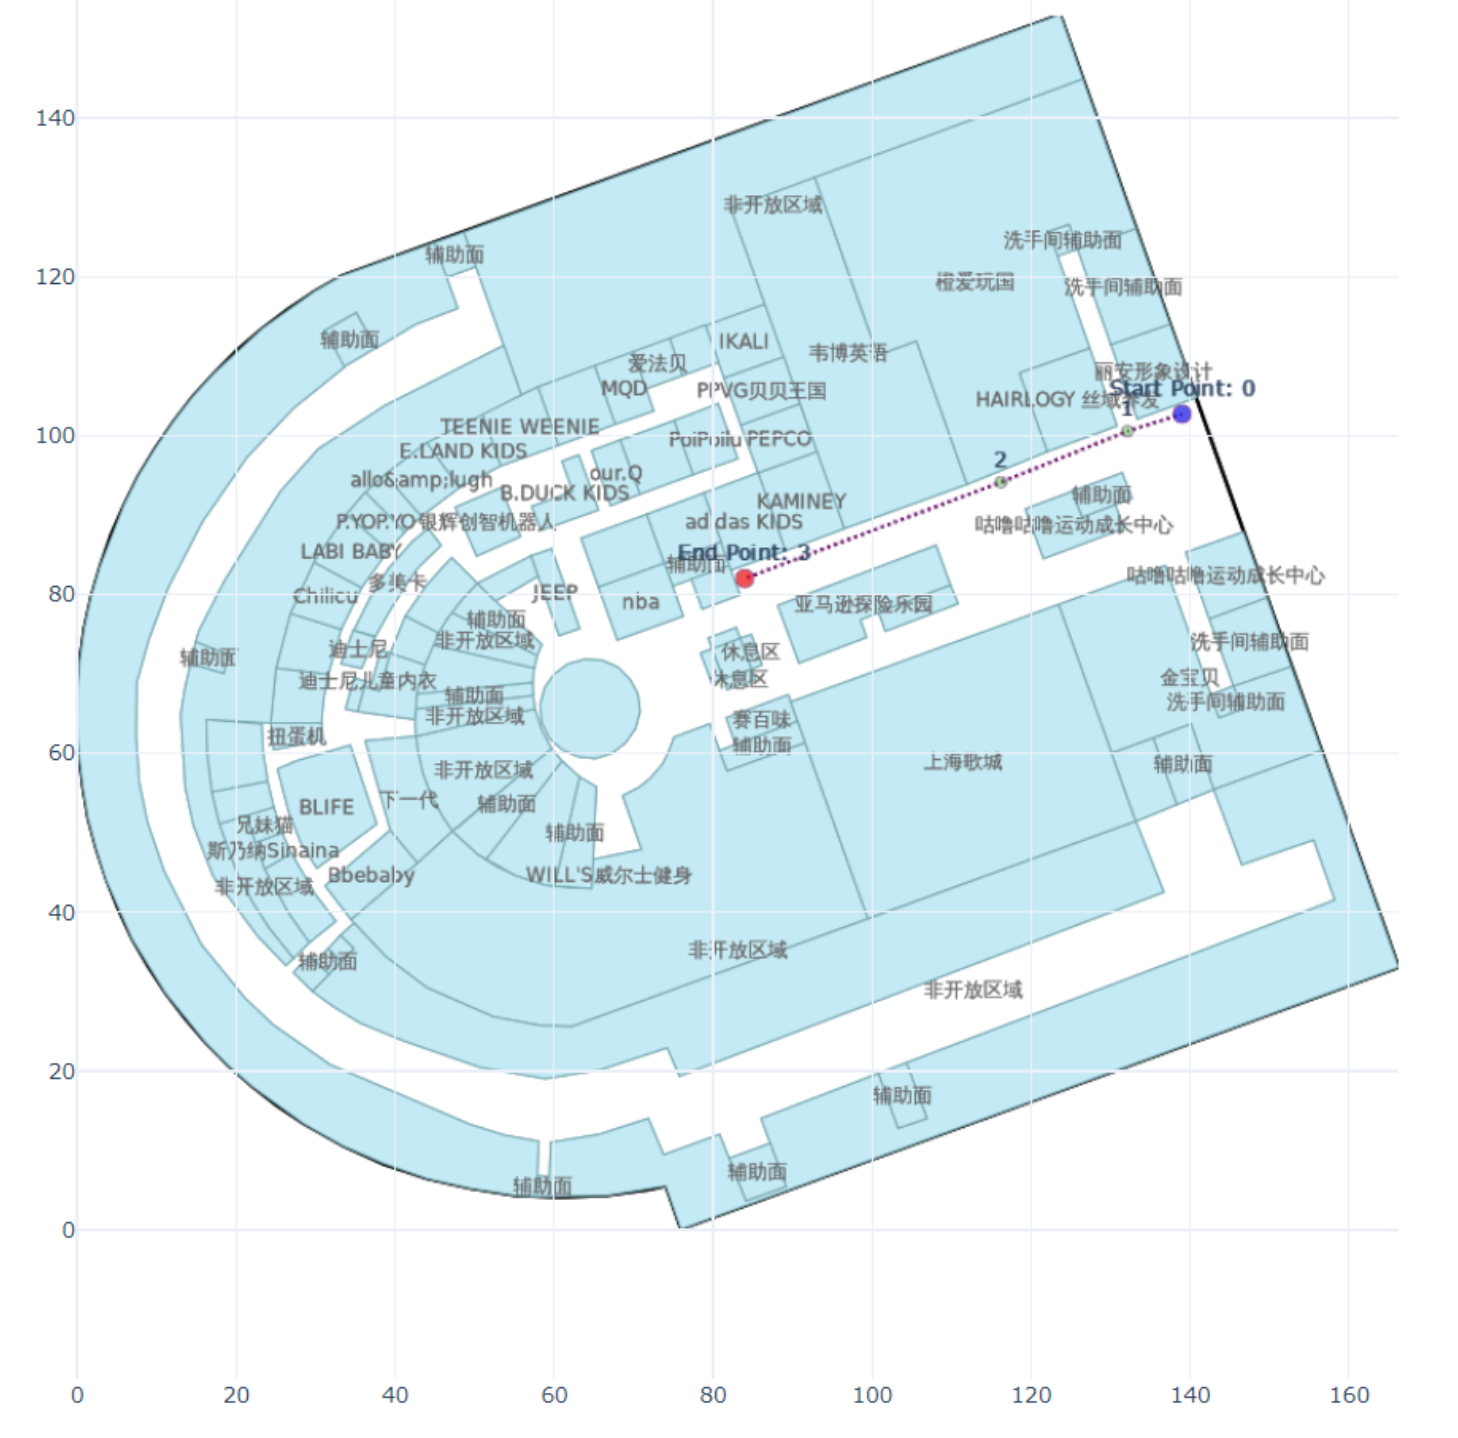
\includegraphics[scale=.37]{Images/ProblemAnalysis/datapath.png}
    \caption{Depiction of a floor with a path from the training data added.}
    \label{fig:datapath}
\end{figure}

It is also possible to view the different paths from the training data on the map of the particular floor. On \textbf{\autoref{fig:datapath}}, we can see the basement floor of the previous figure with one of the paths from the training data. The path on the figure is created from the coordinates of the waypoints (TYPE\_WAYPOINT) in the path file. The blue point is the starting point of the trace and the red point indicates where the path ends. \textbf{\autoref{fig:datapath}} gives an understanding of the distance of a particular path. The different paths vary in size and might cover lesser or larger part of the map. The path given in the figure navigates in a straight line across the room, where other paths can navigate around objects and might trace back to its own starting point.

The training set contains 204 sites. Since we will also have to predict the floor level in addition to the \textit{x} and \textit{y} coordinates, looking into the distribution of floor levels across the training sites could provide insights to whether the class-imbalance problem is present. This problem concerns whether the dataset is well distributed between the classes we want to predict upon. Having a badly distributed dataset could result in the model more often predicting a particular floor level due to a higher occurrence of the aforementioned floor in the dataset, which is not ideal.\cite{Han_Kamber_2012}

\begin{figure}[H]
    \centering
    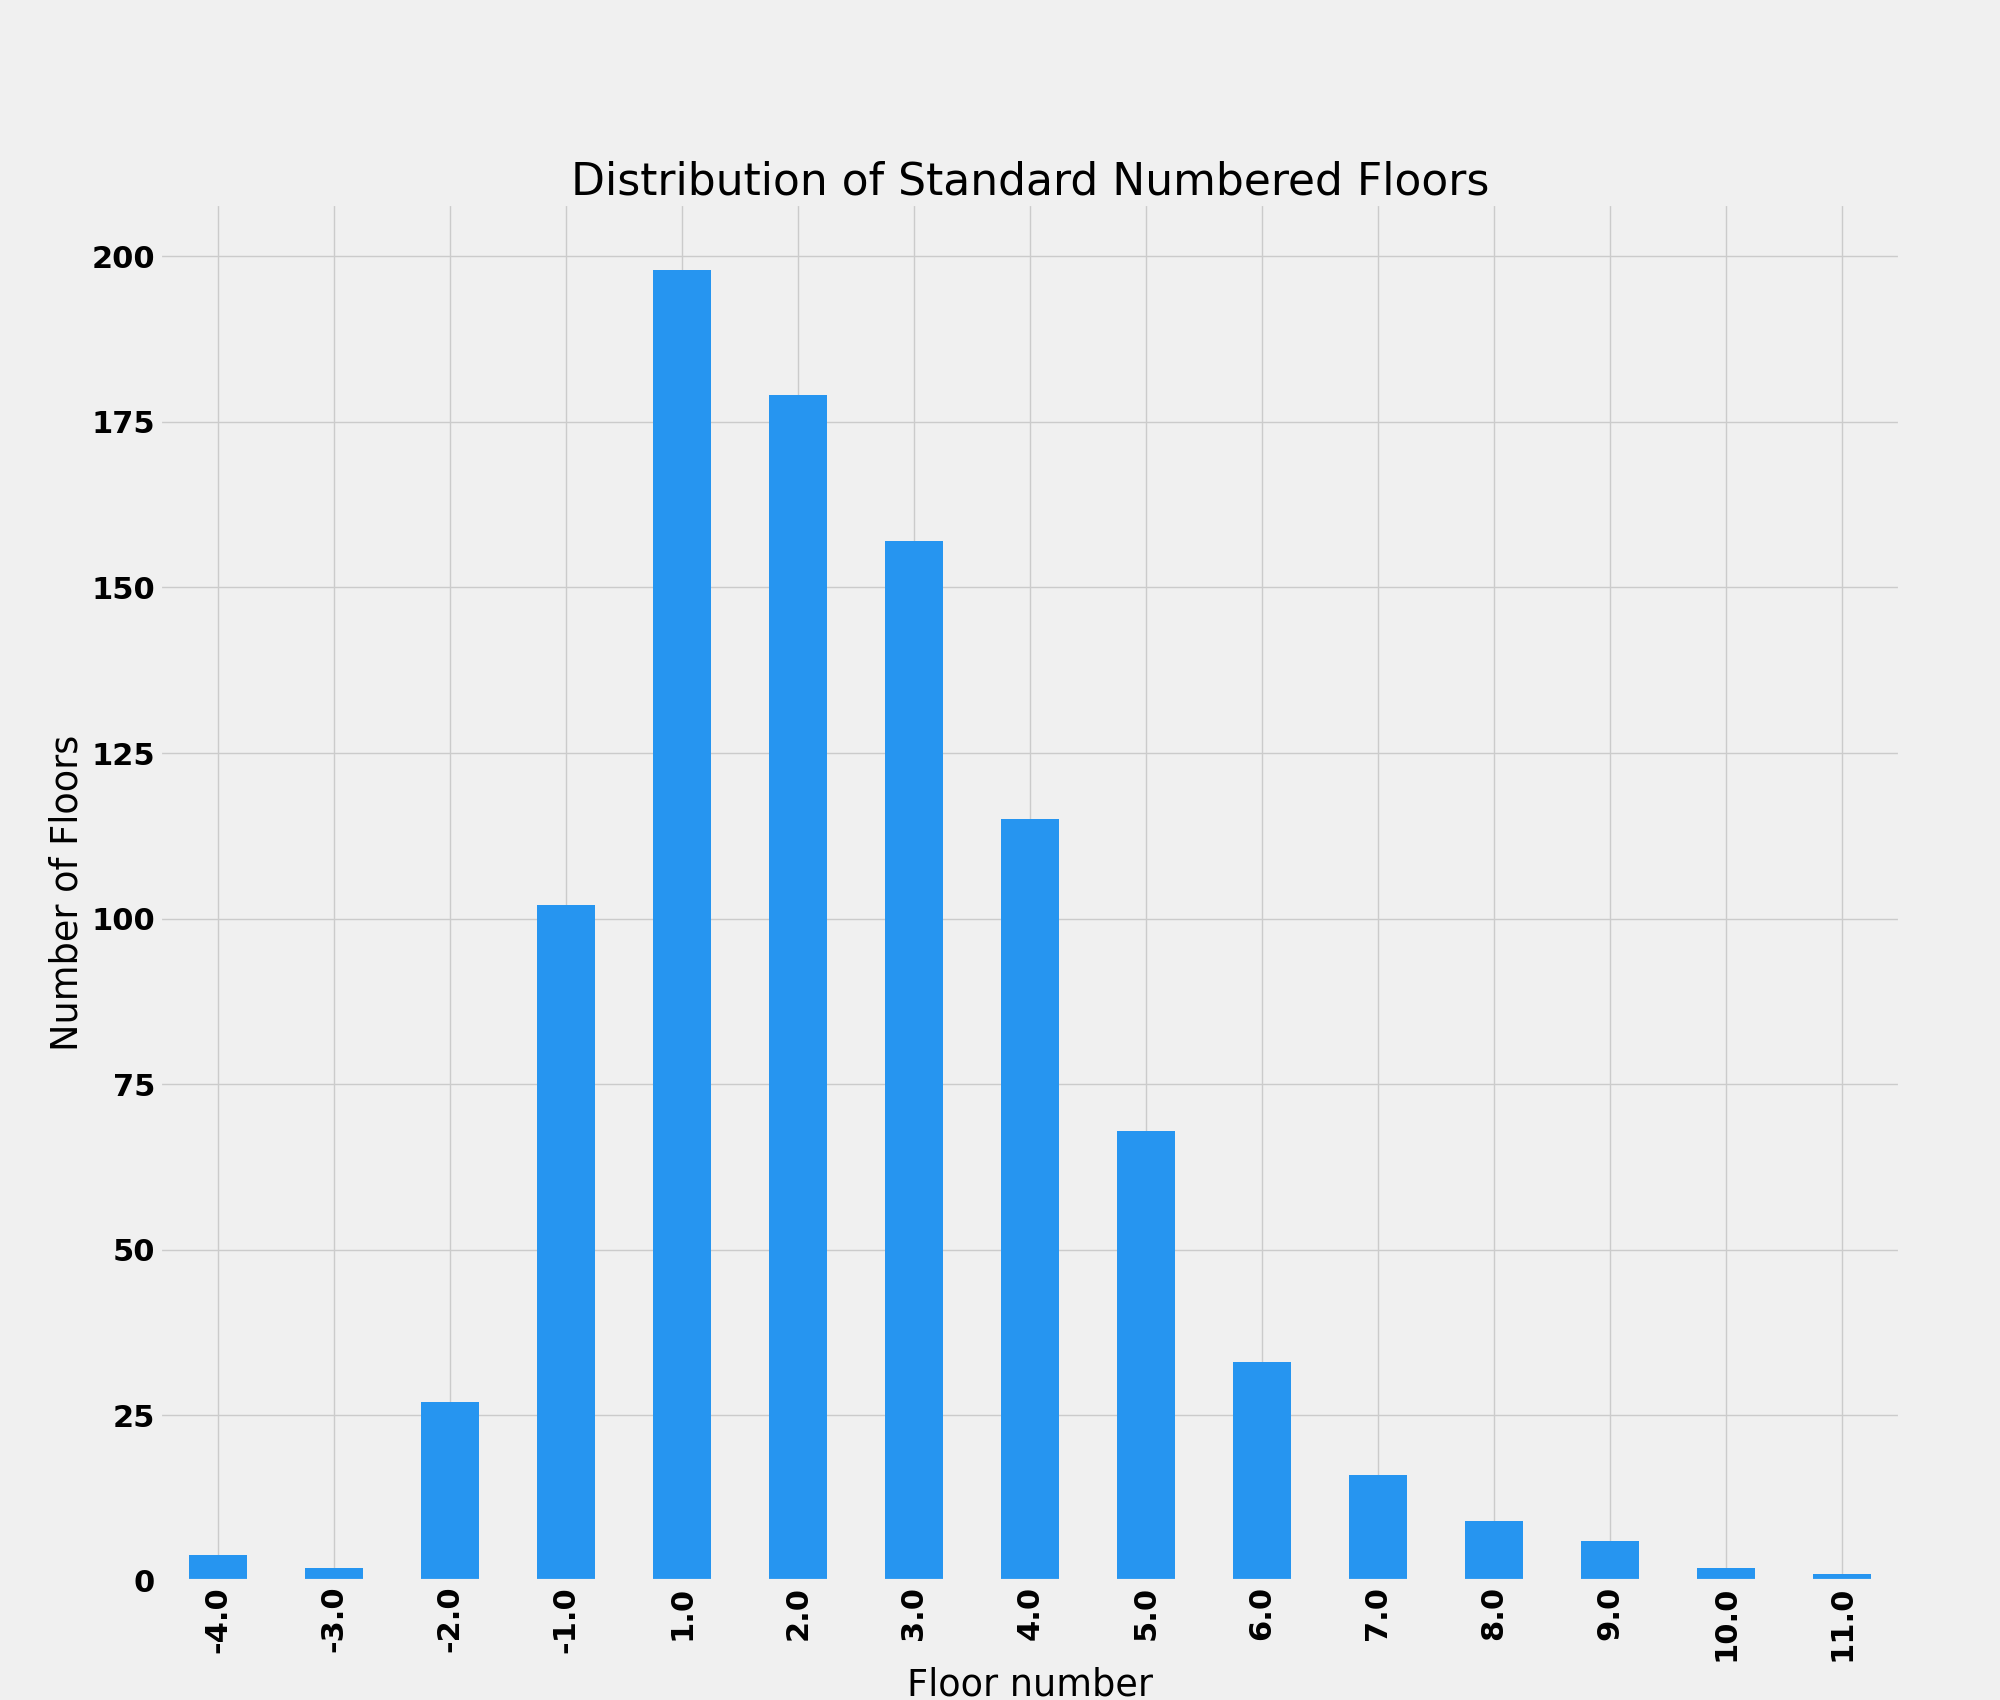
\includegraphics[scale=.15]{Images/ProblemAnalysis/datadistribution1.png}
    \caption{Distribution of standard numbered floors across the data set. X-axis is the floor numbers and y-axis is the number of occurrence of these floors.}
    \label{fig:datadistribution}
\end{figure}

\textbf{\autoref{fig:datadistribution}} displays the number of a particular floor level across the data set. The X-axis denotes the different standard numbered floor levels (positive numbers corresponds to the floors above ground, and the negative numbers corresponds to the basement levels), where the Y-axis describes the number of occurrences of a floor level in the dataset. It is possible from this distribution to see that we possibly have a lot more observations from the floor levels closer to the ground, since they occur more often in the sites in the data set, so this data is also represented in the graph. % Add reason for looking into making an additional distribution on way points per floor.

\begin{figure}[H]
     \centering
     \begin{subfigure}[b]{0.49\textwidth}
         \centering
         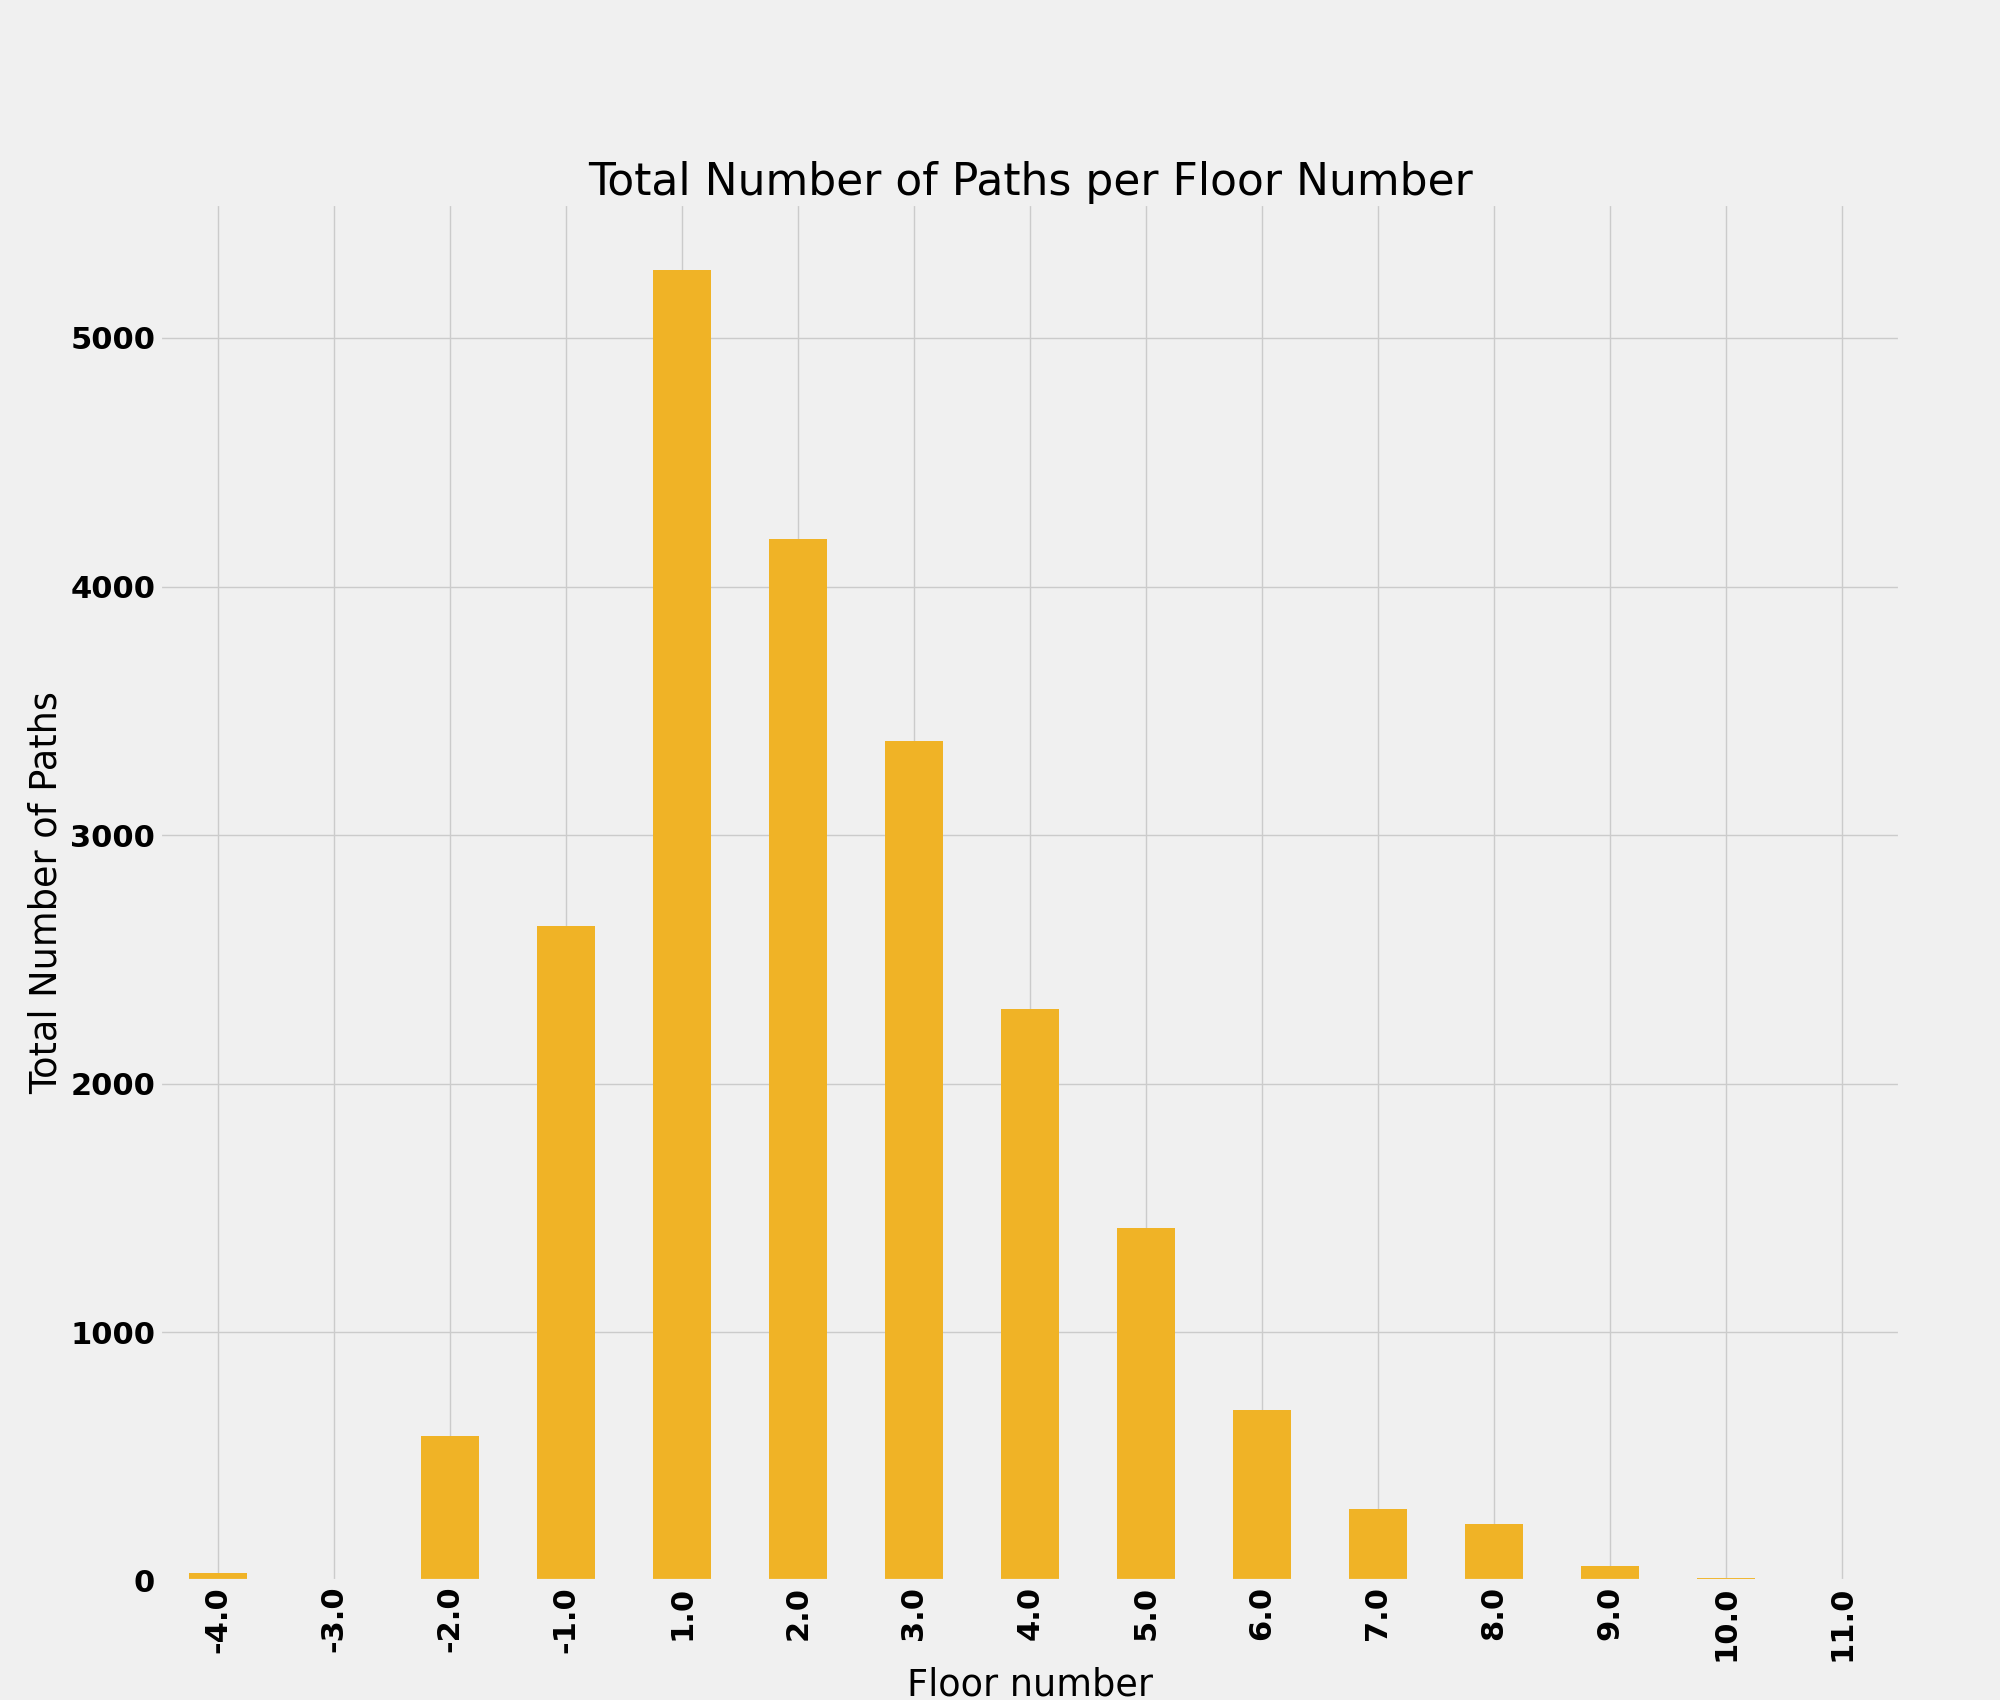
\includegraphics[width=\textwidth]{Images/ProblemAnalysis/datadistribution2.png}
         \caption{Total number of paths per floor number. X-axis is the floor numbers and y-axis is the total numbers of paths on the floors.}
         \label{fig:totalpath}
     \end{subfigure}
     \hfill
     \begin{subfigure}[b]{0.49\textwidth}
         \centering
         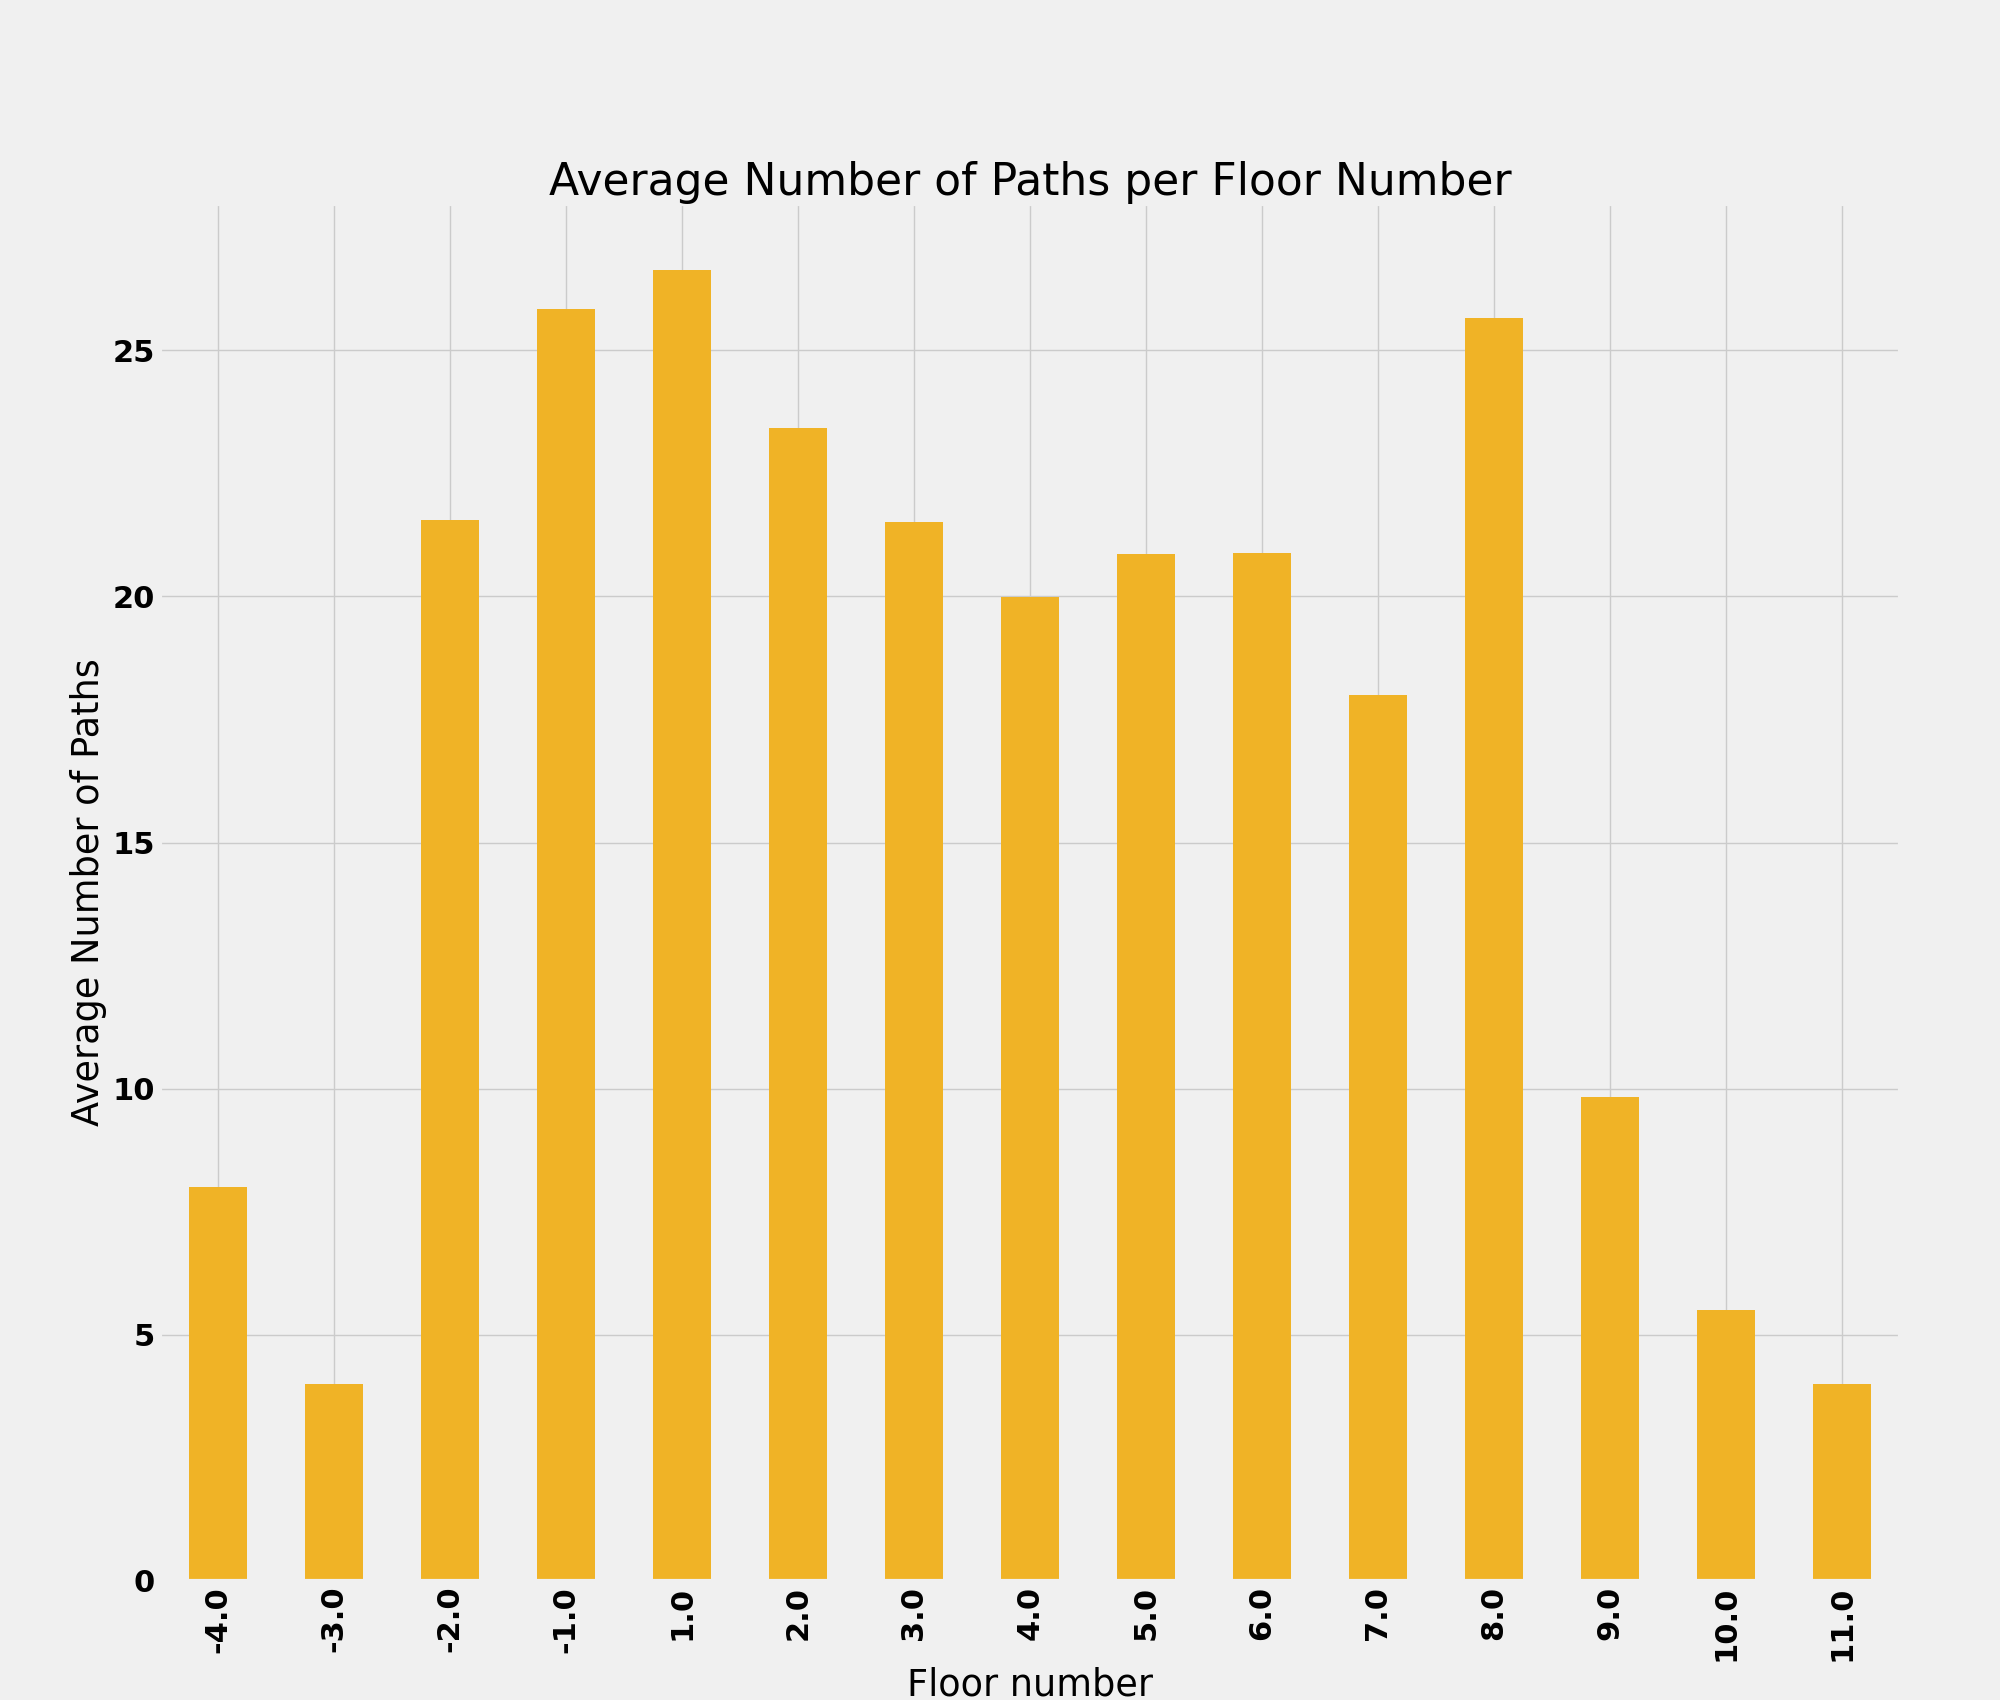
\includegraphics[width=\textwidth]{Images/ProblemAnalysis/datadistribution3.png}
         \caption{Average number of paths per floor. X-axis is the floor numbers and y-axis is the average number of paths on the floor.}
         \label{fig:averagepath}
     \end{subfigure}
        \caption{Distribution of paths in the data set.}
        \label{fig:datadistribution1}
\end{figure}

\textbf{\autoref{fig:datadistribution1}} displays two diagrams of the path distribution in the dataset. In both diagrams, the x-axis denotes floor level and the y-axis describes the number of paths. The first diagram, \textbf{\autoref{fig:totalpath}}, displays the total number of paths across the floor levels, where it is easier to see the difference in occurrences of paths being closer to the ground floor compared to the floors further away. As an example, for the ground floor (F1), we have found 5275 paths across all sites, where for the 10th floor (F11), we only found 4 paths.

Another way to analyse the distribution of paths is to look into the average number of paths for each floor in the dataset. This distribution can be seen on \textbf{\autoref{fig:averagepath}}, which indicates also a large difference between the average number of paths for each floor. A lot of the floors have an average around 20 paths, but floors like the 10th (F11) only have an average of 4 paths.

Alternatively, we can also look into the distribution of waypoints over floors, since the waypoints are the reference locations which will be used to estimate the \textit{x} and \textit{y} coordinates. These distributions can be viewed on \textbf{\autoref{fig:datadistribution2}}.

\begin{figure}[H]
     \centering
     \begin{subfigure}[b]{0.49\textwidth}
         \centering
         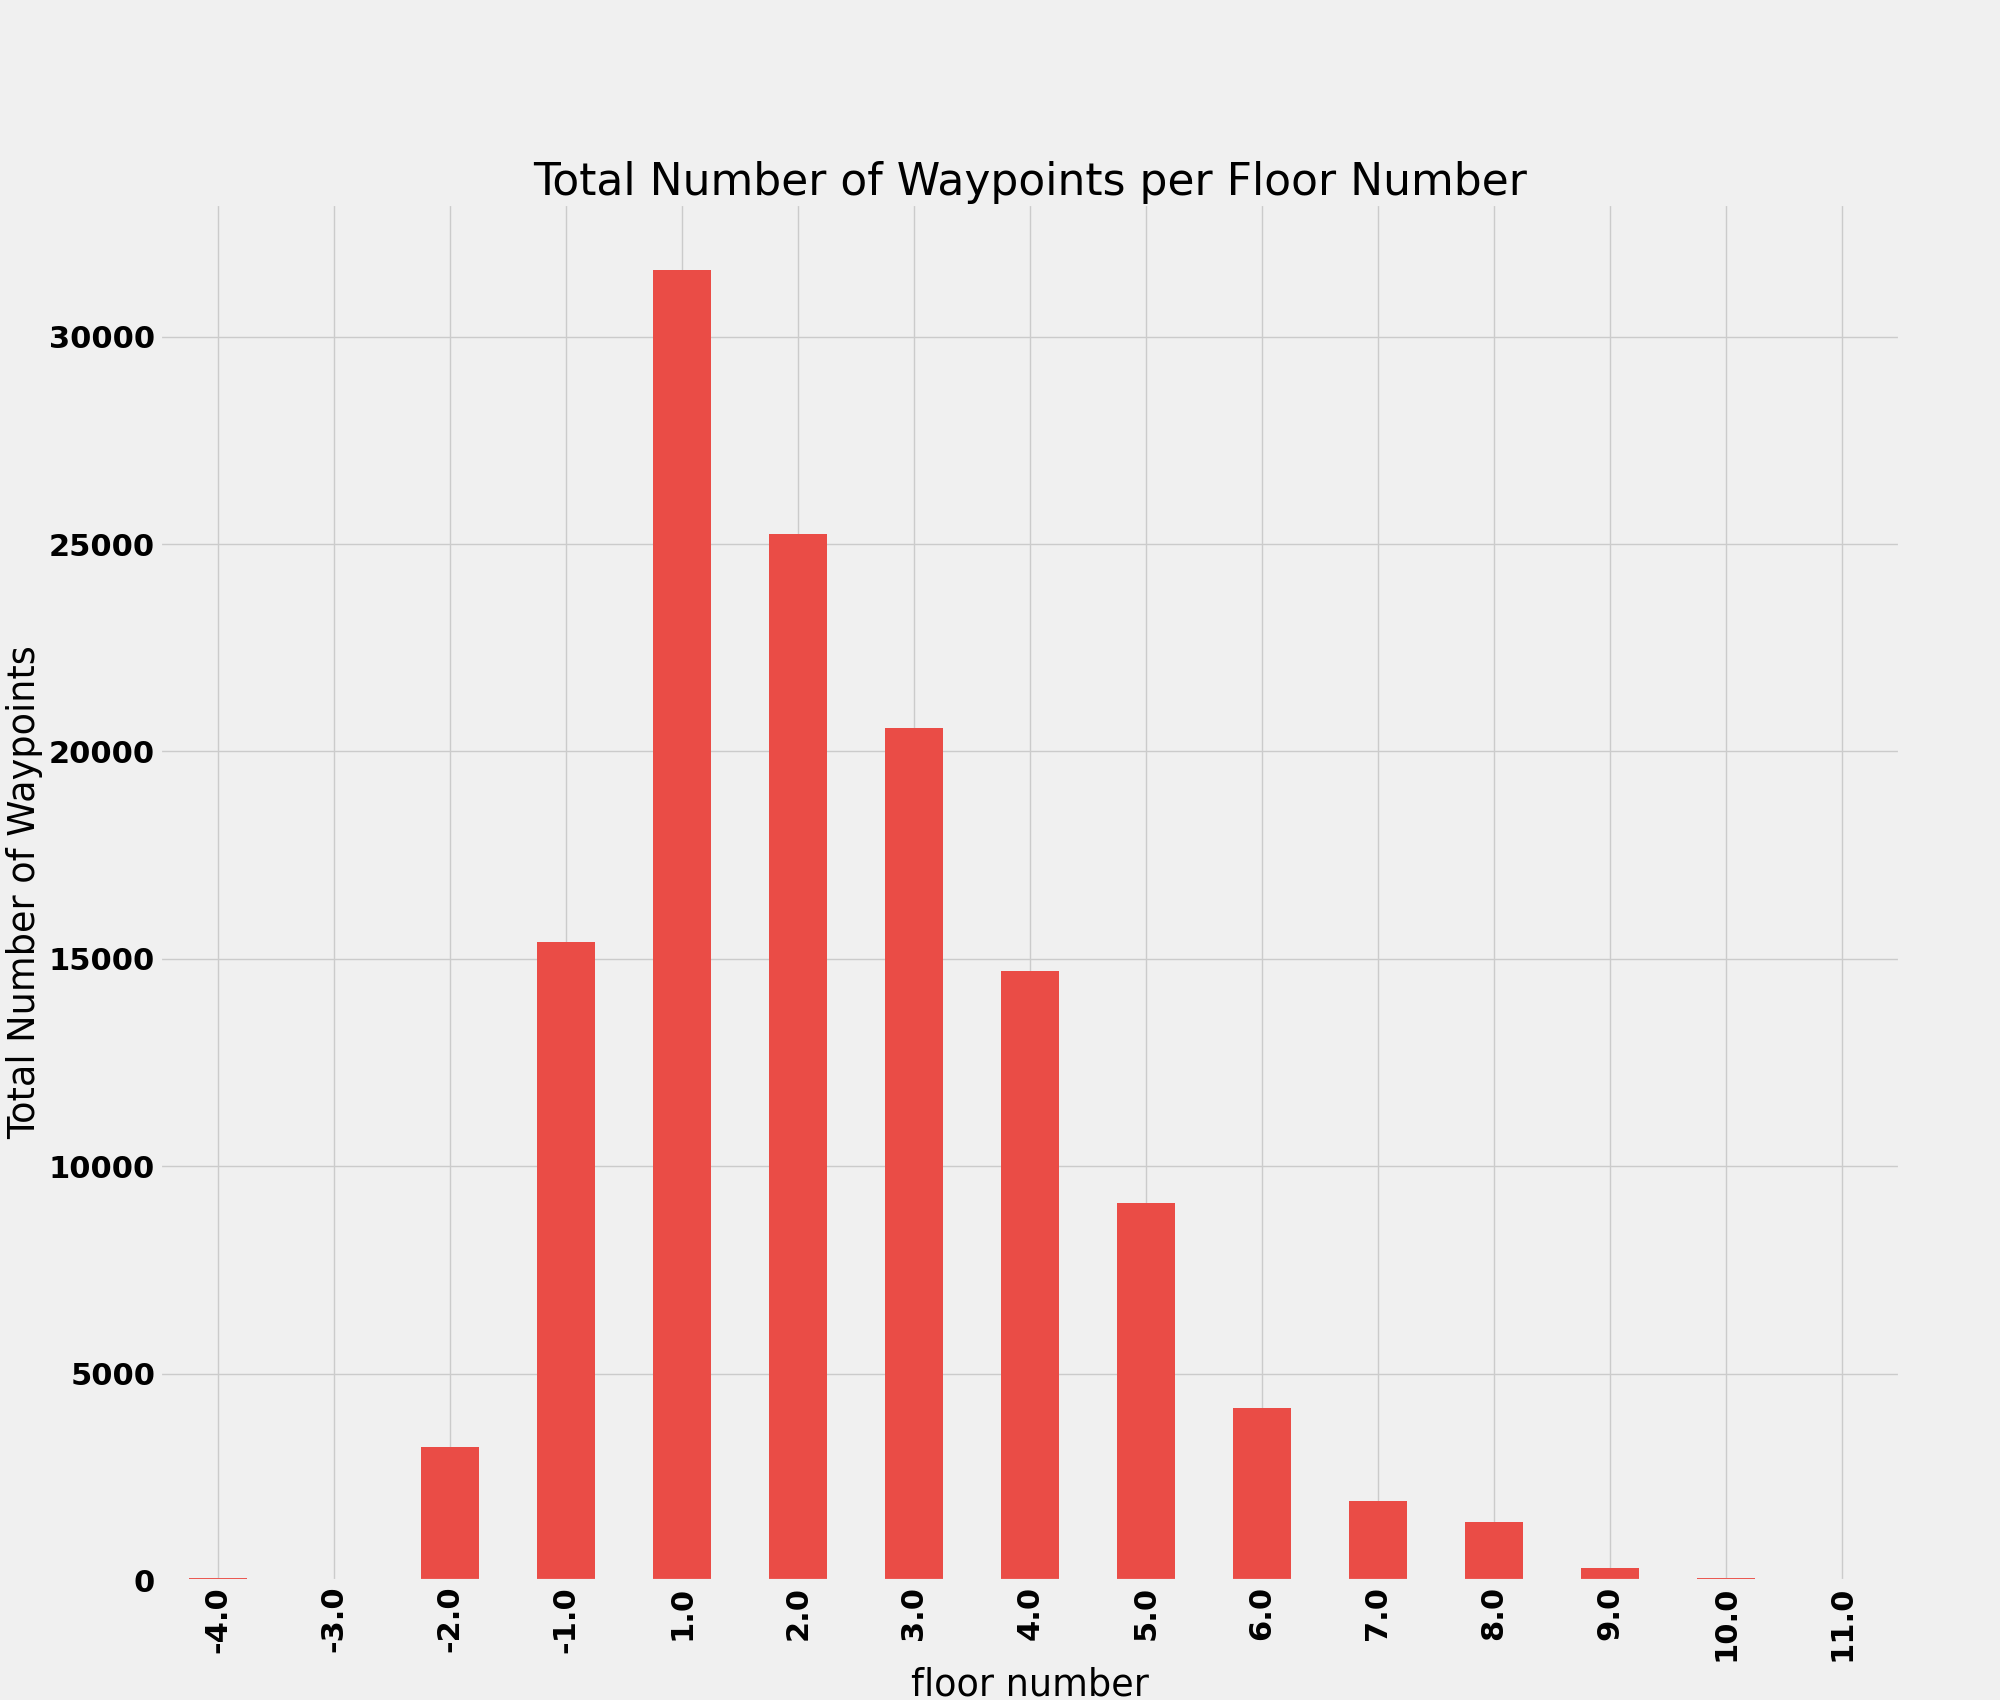
\includegraphics[width=\textwidth]{Images/ProblemAnalysis/datadistribution4.png}
         \caption{Total number of paths per floor number. X-axis is the floor numbers and y-axis is the total numbers of waypoints on the floors.}
         \label{fig:totalwaypoints}
     \end{subfigure}
     \hfill
     \begin{subfigure}[b]{0.49\textwidth}
         \centering
         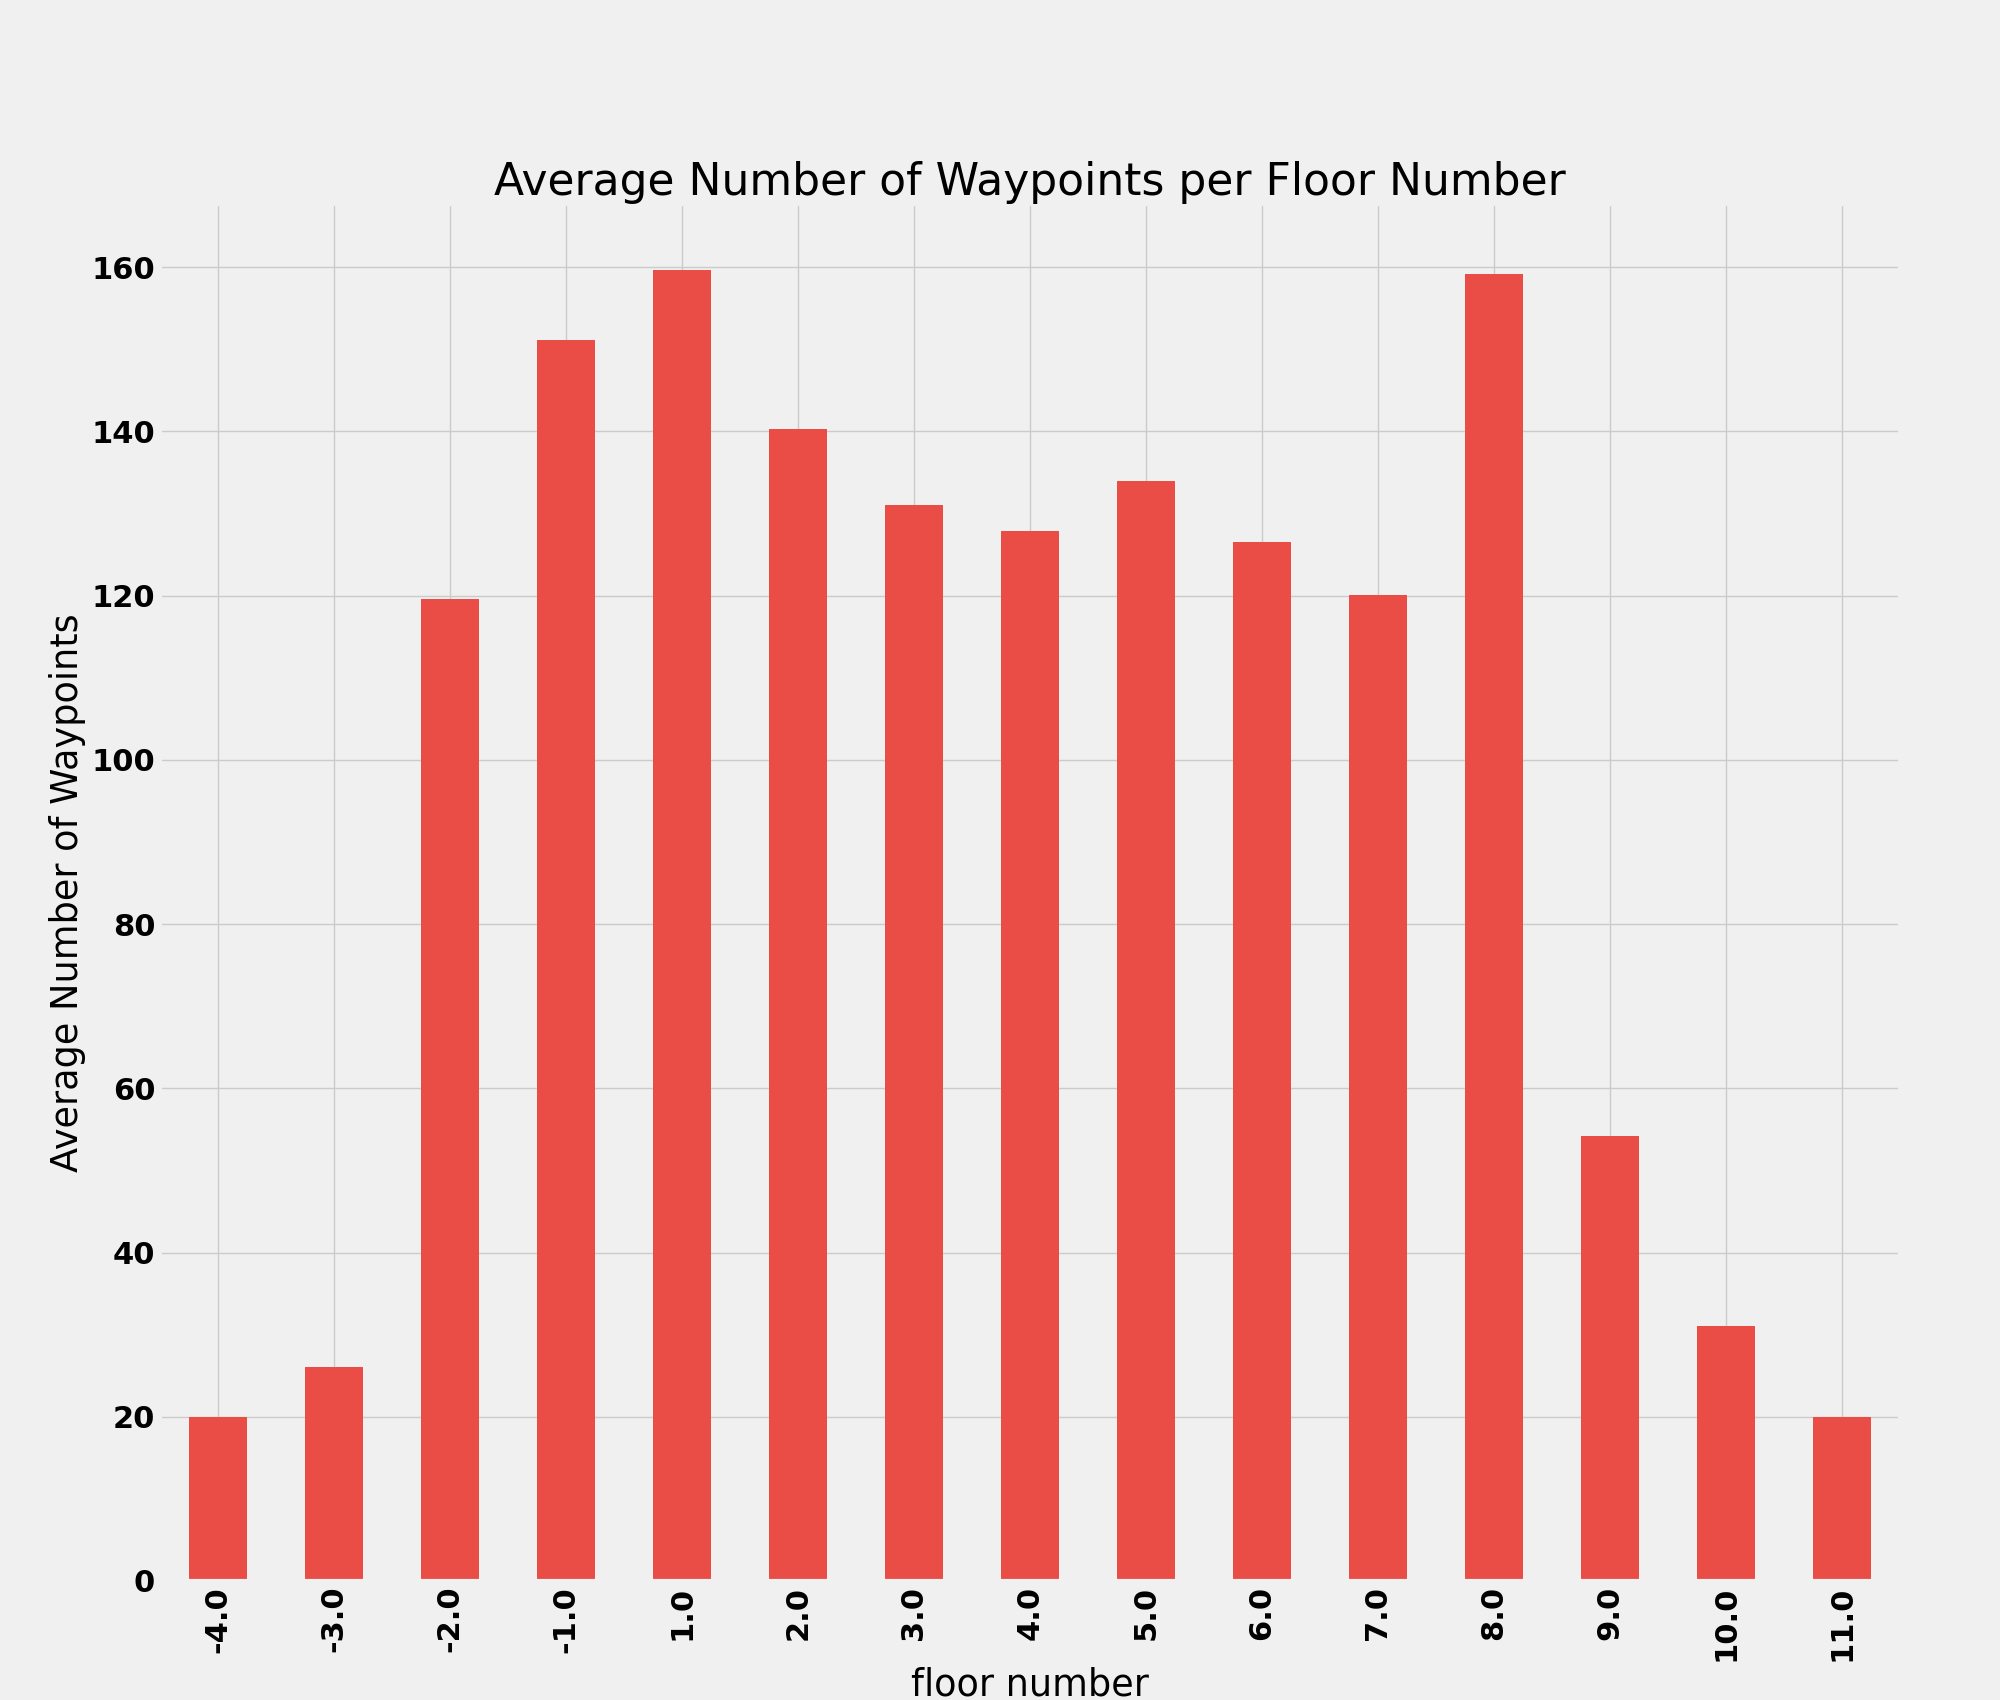
\includegraphics[width=\textwidth]{Images/ProblemAnalysis/datadistribution5.png}
         \caption{Average number of paths per floor. X-axis is the floor numbers and y-axis is the average number of waypoints on the floor.}
         \label{fig:averagewaypoints}
     \end{subfigure}
        \caption{Distribution of waypoints in the data set.}
        \label{fig:datadistribution2}
\end{figure}

\textbf{\autoref{fig:totalwaypoints}} displays the number of waypoints for each floor. The distribution is looking quite similar to \textbf{\autoref{fig:totalpath}}, which could indicate a similar amount of waypoints for each path. To ensure this hypothesis we decided to look into the average number of waypoints per floor as seen on \textbf{\autoref{fig:averagewaypoints}}. This yielded a bit different distribution compared to \textbf{\autoref{fig:averagepath}}, where we can see that the 4th basement level (-4 or B4) has a quite lower average in waypoints per floor than paths per floor, which indicates having more paths but with lesser waypoints in them.

%The test set contains 626 paths to predict upon.


% Måske tjekke distribution på antallet af entries for de forskellige floors.
% boxplot over number of levels (lowest/highest)
%Cleaning the data based on the previous section - maybe even the distribution



%\subsection{Data Cleaning}




